\documentclass[14pt]{extarticle}
\usepackage[utf8]{inputenc}
\usepackage[T1]{fontenc}
\usepackage[spanish,es-lcroman]{babel}
\usepackage{amsmath}
\usepackage{amsthm}
\usepackage{physics}
\usepackage{tikz}
\usepackage{float}
\usepackage[autostyle,spanish=mexican]{csquotes}
\usepackage[per-mode=symbol]{siunitx}
\usepackage{gensymb}
\usepackage{multicol}
\usepackage{enumitem}
\usepackage{caption}
\captionsetup[table]{skip=5pt}
\usepackage[left=2.00cm, right=2.00cm, top=2.00cm, 
     bottom=2.00cm]{geometry}

%\renewcommand{\questionlabel}{\thequestion)}
\decimalpoint
\sisetup{bracket-numbers = false}

\title{\vspace*{-2cm} Práctica 7 - Medición de temperatura \\  Física III \vspace{-5ex}}
\date{}

\begin{document}
\maketitle
\renewcommand{\tablename}{Tabla}

\section{Trabajo a realizar.}

Luego de haber realizado las mediciones de ascenso y descenso de temperatura para el agua y el agua con sal, la siguiente etapa de trabajo es discutir los resultados.

\begin{enumerate}
\item  Prepara los datos en tablas para una mejor lectura, como se espera que tengan un número considerable de pares de datos, pueden aprovechar el espacio de la hoja, para acomodar las tablas:

\vspace*{1cm}
Agua. \hspace{0.5cm} Temperatura inicial: \rule{2cm}{0.1mm} \\[0.5em]
Agua con sal. \hspace{0.5cm} Temperatura inicial: \rule{2cm}{0.1mm}

\vspace*{0.25cm}
\begin{minipage}[t]{0.45\linewidth}
\begin{table}[H]
\centering
\caption{Ascenso: agua}
\begin{tabular}{| c | c |} \hline
Temperatura [\si{\degreeCelsius}] & tiempo [\si{\second}] \\ \hline
 & \num{15} \\ \hline
 & \num{30} \\ \hline
 & \num{45} \\ \hline
\vdots & \vdots \\ \hline
\end{tabular}
\end{table}
\end{minipage}
\begin{minipage}[t]{0.45\linewidth}
\begin{table}[H]
\centering
\caption{Ascenso: agua con sal}
\begin{tabular}{| c | c |} \hline
Temperatura [\si{\degreeCelsius}] & tiempo [\si{\second}] \\ \hline
    & \num{15} \\ \hline
    & \num{30} \\ \hline
    & \num{45} \\ \hline
\vdots & \vdots \\ \hline
\end{tabular}
\end{table}
\end{minipage}

\vspace{1.5cm}

\begin{minipage}[t]{0.45\linewidth}
\begin{table}[H]
\centering
\caption{Descenso: agua}
\begin{tabular}{| c | c |} \hline
Temperatura [\si{\degreeCelsius}] & tiempo [\si{\second}] \\ \hline
    & \num{15} \\ \hline
    & \num{30} \\ \hline
    & \num{45} \\ \hline
\vdots & \vdots \\ \hline
\end{tabular}
\end{table}
\end{minipage}
\begin{minipage}[t]{0.45\linewidth}
\begin{table}[H]
\centering
\caption{Descenso: agua con sal}
\begin{tabular}{| c | c |} \hline
Temperatura [\si{\degreeCelsius}] & tiempo [\si{\second}] \\ \hline
    & \num{15} \\ \hline
    & \num{30} \\ \hline
    & \num{45} \\ \hline
\vdots & \vdots \\ \hline
\end{tabular}
\end{table}
\end{minipage}
\item Completa la siguiente tabla en donde se van a reportar el total de datos obtenidos y el tiempo total de registro para cada solución:

\begin{table}[H]
\centering
\begin{tabular}{|l | c | c | c | c | } \hline
 & \multicolumn{2}{ c |}{Ascenso} & \multicolumn{2}{ c |}{Descenso} \\ \hline
Solución & Datos & Tiempo & Datos & Tiempo \\ \hline
Agua & & & & \\ \hline
Agua con sal & & & & \\ \hline
\end{tabular}
\end{table}
\item Prepara la gráfica de la siguiente forma: el eje de las abscisas será el eje para el tiempo en segundos, mientras que para el eje de las ordenadas, se tendrá el valor de temperatura. En este apartado te puedes apoyar con programas tipo Excel, que te facilitarán el manejo de los datos; también puedes hacer la gráfica a mano.
\begin{figure}[H]
\centering
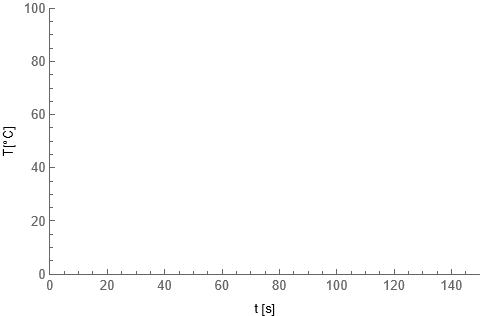
\includegraphics[scale=0.8]{Imagenes/Calor_01.png}
\end{figure}
Es importante que NO unas los puntos experimentales, debe de aparecer solo la marca de cada par ordenado.
\item En una misma gráfica deben de estar los datos de ascenso de temperatura del agua y del agua con sal, usa una marca distinta o un color distinto para diferenciarlos.
\item Entonces debes de preparar dos gráficas: a) una de ascenso (con las dos soluciones), b) una de descenso con las dos soluciones.
\item Esto es lo que se va a discutir en la siguiente clase:
\begin{enumerate}
\item ¿Cuál de las dos soluciones llega más rápido a la ebullición? ¿Por qué?
\item ¿Cuál de las dos soluciones se enfría más rápido? ¿Por qué?
\end{enumerate}
Deberás de preparar las respuestas que presentarás en la clase de Laboratorio.
\end{enumerate}

\end{document}